%
\documentclass[english]{article}
%%%%%%%%%%%%%%%%%%%%%%%%%%%%%%%%%%%%%%%%%%%%%%%%%%%%%%%%%%%%%%%%%%%%%%%%%%%%%%%%%%%%%%%%%%%%%%%%%%%%%%%%%%%%%%%%%%%%%%%%%%%%
\usepackage{latexsym,amsmath,amssymb,amsfonts,fullpage,graphicx,placeins}
\usepackage[capposition=top]{floatrow}

\begin{document}
Gabrielle Merritt 
\\
gmerritt@seas.upenn.edu 
\begin{center}
{\textbf{ESE 505 Homework 4}} \\
\end{center}
\section*{Transfer Function from Points}
\subsection*{A}
\begin{figure}[!ht]
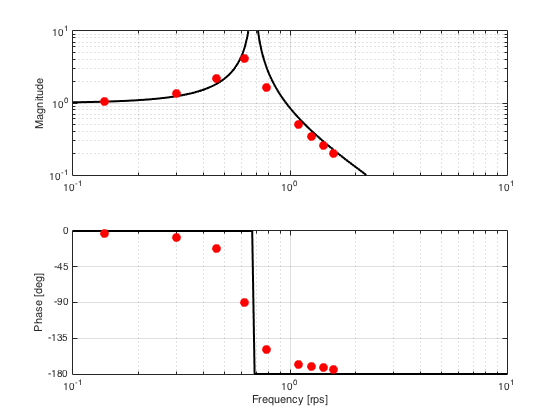
\includegraphics[width = \linewidth]{frqA.png}
\label{fig:1_a}
\caption{Find Transfer Function from Simulink}
\end{figure}
\subsection*{B}
\begin{figure}[!ht]
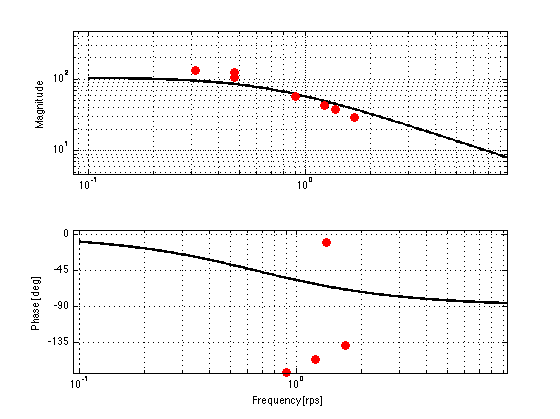
\includegraphics[width = \linewidth]{frqB.png}
\label{fig:1_a}
\caption{Find Transfer Function from Simulink}
\end{figure}
\FloatBarrier
\section*{Creating Bode Plots from Transfer Functions}
\subsection{$G(s) = \frac{1000}{s + 200} $}
\begin{figure}[!ht]
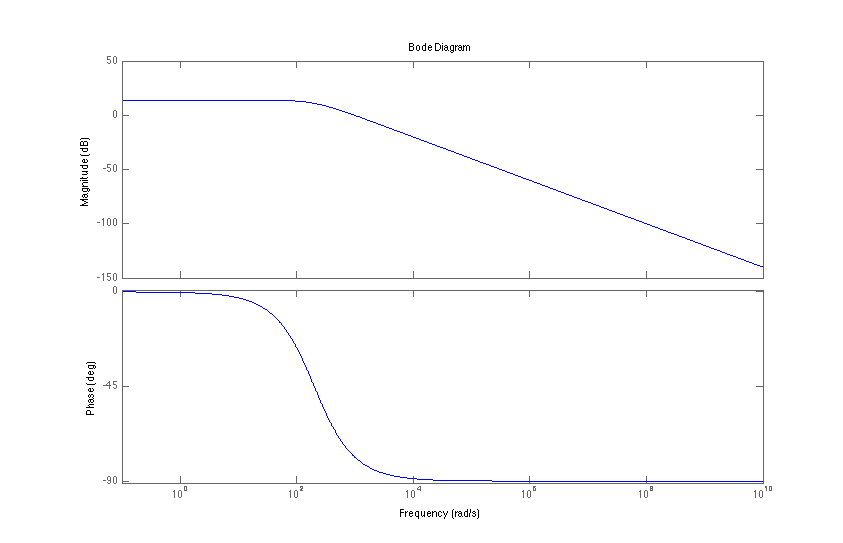
\includegraphics[width = \linewidth]{2a.png}
\label{fig:2_a}
\caption{Bode plot of $G(s) = \frac{1000}{s + 200} $}
\end{figure}
\FloatBarrier

\subsection{$G(s) = \frac{9s +27}{(s+1)^2+ (s^2 +3s +81)} $}
\begin{figure}[!ht]
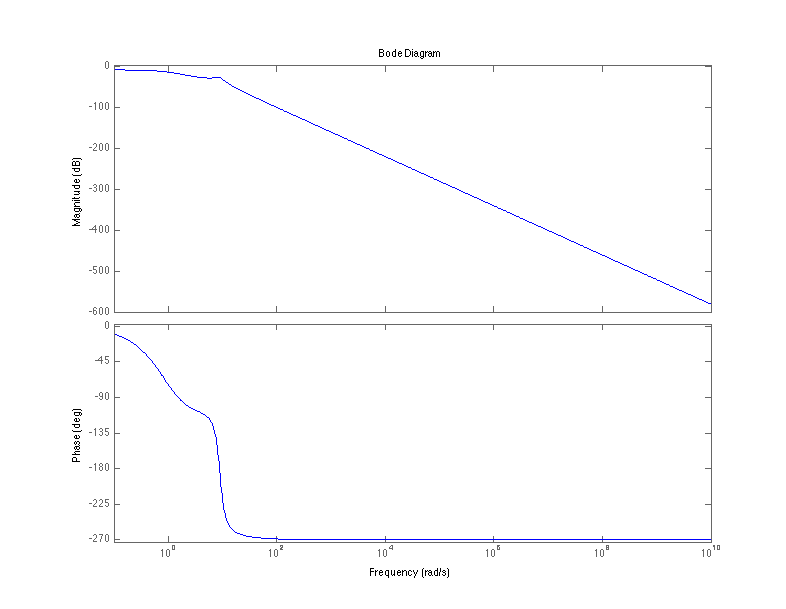
\includegraphics[width = \linewidth]{2b.png}
\label{fig:2_b}
\caption{Bode plot of $G(s) = \frac{9s +27}{(s+1)^2+ (s^2 +3s +81)} $}
\end{figure}
\FloatBarrier

\subsection{$G(s) = \frac{100s}{ (s^2 +s +25)} $}
\begin{figure}[!ht]
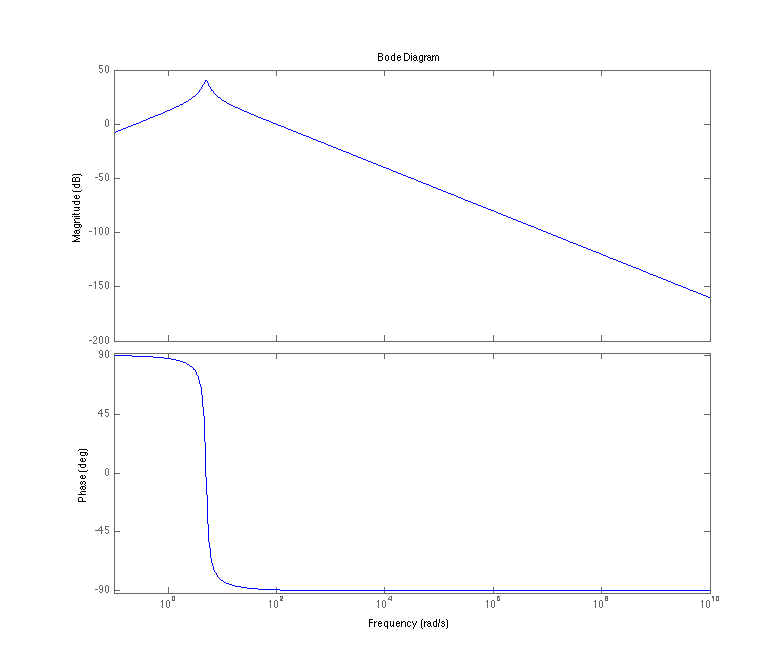
\includegraphics[width = \linewidth]{2c.png}
\label{fig:2_c}
\caption{Bode plot of $G(s) = \frac{100s}{ (s^2 +s +25)} $}
\end{figure}
\FloatBarrier

\subsection{$G(s) = \frac{2000s + 2000}{ (s(s+10)(s+100)} $}
\begin{figure}[!ht]
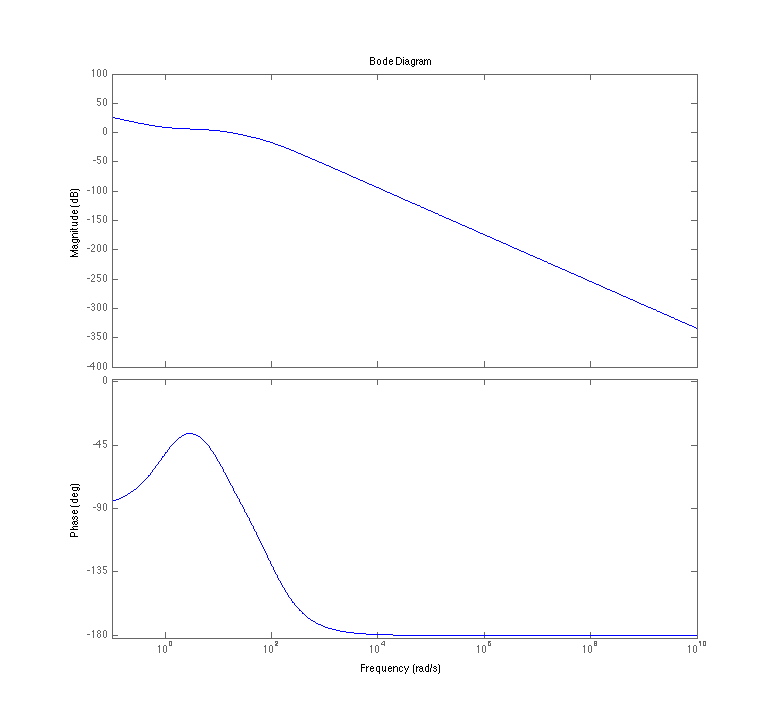
\includegraphics[width = \linewidth]{2d.png}
\label{fig:2_d}
\caption{Bode plot of$G(s) = \frac{2000s + 2000}{ (s(s+10)(s+100)} $}
\end{figure}
\FloatBarrier

\section*{Controller Design}
	\subsection*{Ziegler Nicholas Ultimate Sensitivity Form}
	Zigerler Nichols form can be writter as  
	$$ KG_c = K_p + \frac{K_d }{s}+K_is $$
	$$K_p = .6 *K_u ,  K_d = \frac{2K_p}{T_u s} , K_i  = \frac{K_pT_u s}{8} $$ 
	$$ KG_c = .6K_u \big( \frac{2}{T_us} + \frac{T_u s}{8} \big) $$
	$$KG_C = \frac{.6K_u}{8T_u} \big( \frac{16 + s^2 T_u^2}{s} \big) $$  
	$$KG_C =\frac{.6K_u}{8T_u}\bigg( \frac{(T_us +4)^2}{s} \bigg) $$    
	
	\subsection*{Proportional Feed Back}
	Using a root locus with proportional feed back only we found that our $K_u$ = 30. and our $\omega_d$ = 2.23, which when converted to find $T_u$ = 2.8.   Using these values to plug in for $K_u$ and$T_u$, in our compensator function we have $K$ = 6.3 and $a$ = 1.4. 
When we plot the root locus of our transfer function with our PID controller included we have: 
\begin{figure}[h!]
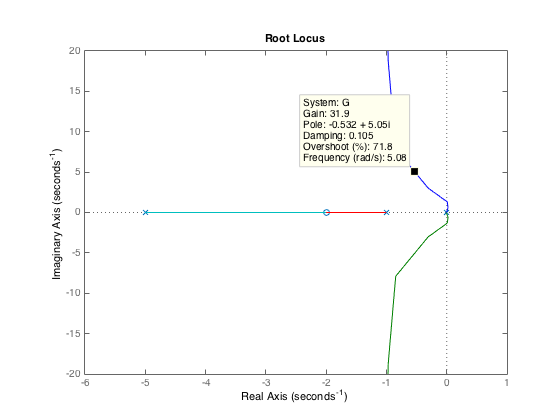
\includegraphics[width = \linewidth]{32gain_a2.png}
\label{fig:3_a}
\caption{Root locus with PID controller}
\end{figure}
\FloatBarrier
\subsection*{ Using only Proportional feedback  make a bode plot of $KG_cG_p(s)$ with K = 5 . What is the gain
margin for this system? }
For the system$KG_cG_p(s)$ we get use the transfer function 
$$
\frac{K}{s(s +1)(s+5}
$$
Which gives us the following bode plot:
\begin{figure}[h!]
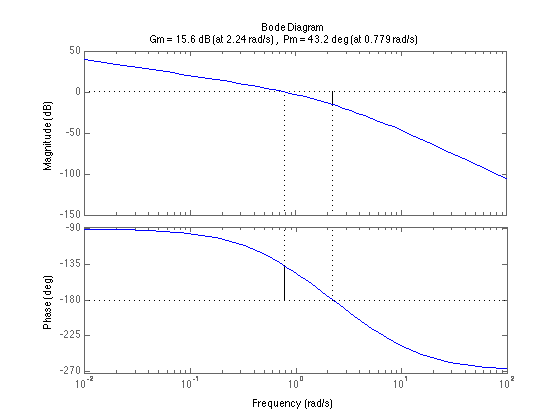
\includegraphics[width = \linewidth]{3c2.png}
\caption{Bode Plot of Transfer function with only proportional gain }
\label{fig:3_c}
\end{figure}

As you can see in~\ref{fig:3_c} We have  a gain margin of ~15.6 dB, which is close to a magnitude of 6. So we can say that we can increase the gain by a factor of 5 to reach neutral stability. Like wise we see that $\omega_phase$ is the same as the previous problem which implies the neutrally stable period of 2.28 seconds. 
\FloatBarrier

\subsection*{ Bode plot of $KG_cG_p(s)$ , for the Ziegler-Nichols design with the nominal gain.}
Replacing K with the $\frac{.6K_u}{8T_u}\bigg( \frac{(T_us +4)^2}{s} \bigg)$
We have the new transfer function  
$$
\frac{.6K_u}{8T_u}\bigg( \frac{(T_us +4)^2}{s} \bigg) \frac{1}{s(s +1)(s+5}
$$
In figure~\ref{fig:3_d} We see that we have an infinite Gain margin because the system is stable for all values of K, and therefore never pass -180 degrees on the phase plot 

\begin{figure}[h!]
\caption{ Bode plot of  Open loop Transfer function with PID controller}
\label{fig:3_d}
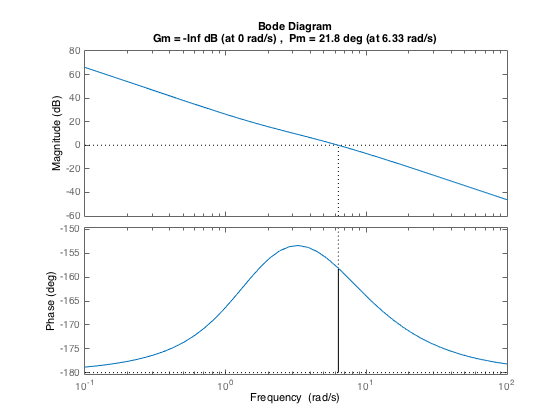
\includegraphics[width=\linewidth]{3d2.png}
\end{figure} 
\FloatBarrier
\subsection*{find a value for a that would allow for 45 degrees of phase margin. What is the value of K that achieves this margin? Submit the bode plot that shows these values.}
For this part I tried different values of a  and saw how the phase margin shifted. For a = 0 Figure~\ref{fig:3_e1}  we have an infinite phase and gain margin (gain never crosses 0 dB) and a maximum possible phase margin of 25 degrees
\begin{figure}[h!]
\caption {Bode plot of open loop transfer function PID with a =0} 
\label{fig:3_e1}
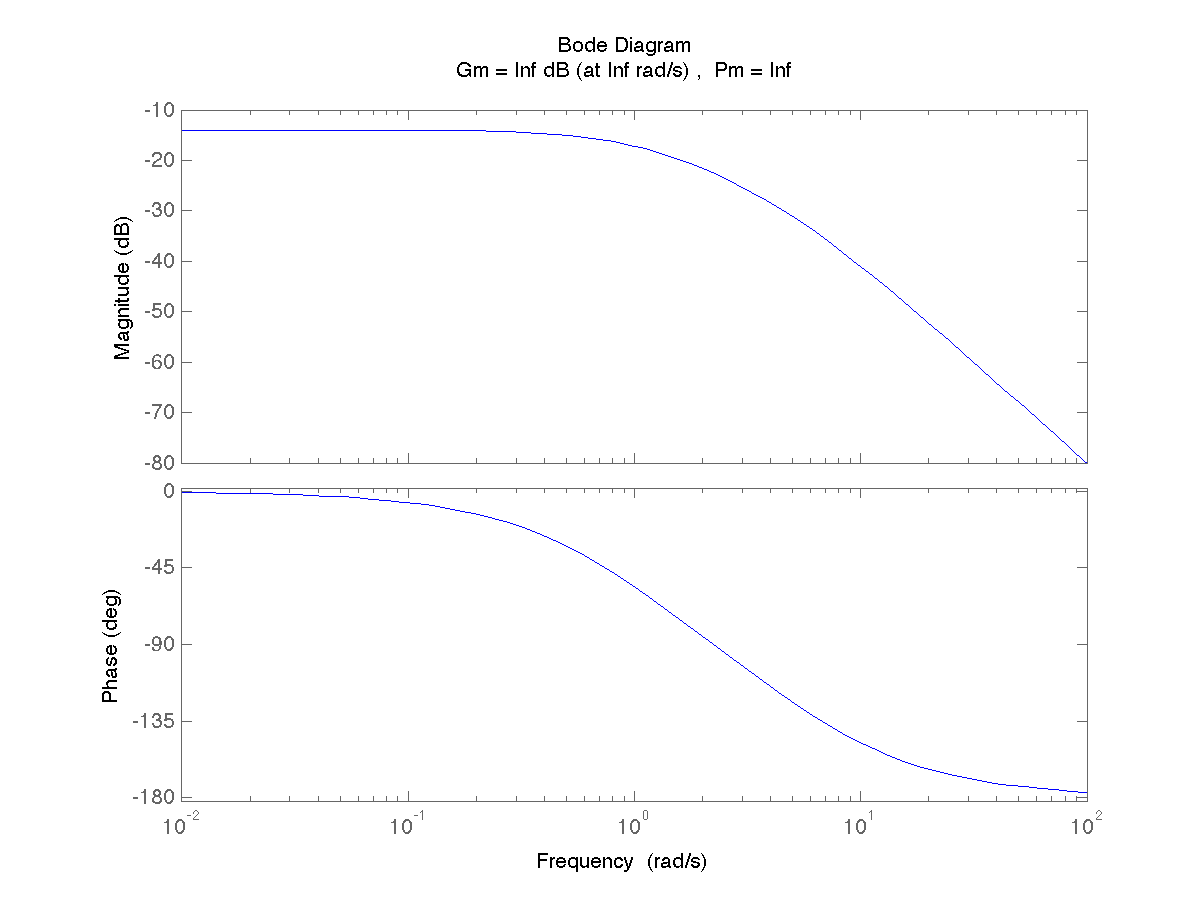
\includegraphics[width =\linewidth]{3e_a0.png}
\end{figure} 
\FloatBarrier
So I increased a to be .5 in figure~\ref{fig:3_e2} we see that we now have a maximum possible margin of 71 degrees 
\begin{figure}[h!]
\caption{Bode plot of open loop transfer function PID with a = .5} 
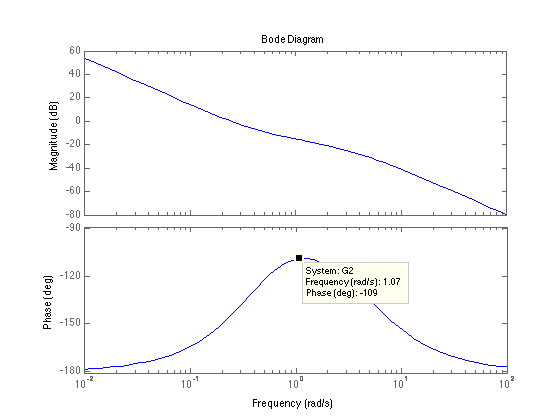
\includegraphics[width = \linewidth]{3e_ahalf2.png}
\label{fig:3_e2}
\end{figure}
\FloatBarrier
The closest to the 45 degree maximum phase angle turned out to be a = .9 
as seen in figure~\ref{fig:3_e3}. 
\begin{figure}[h!]
\caption{Bode plot of open loop transfer function PID with a = .9} 
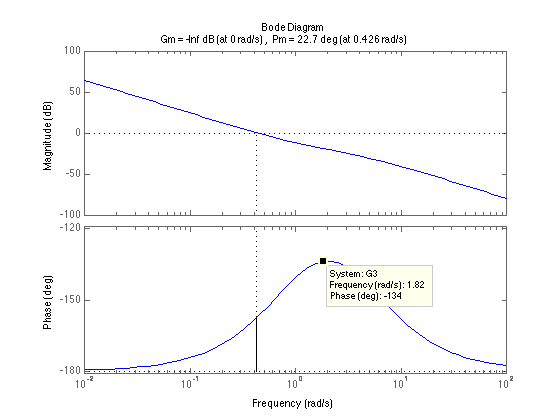
\includegraphics[width = \linewidth]{3e_apoint9.png}
\label{fig:3_e3}
\end{figure}
\FloatBarrier

\section*{Apply frequency-response analysis to the Black-Box system.}
\subsection{Bode plots of Analog and Digital System}
For the Black box system for both the analog and digital implementations we can look at the gain margin to find our $K_u$ and our $\omega_phase$ to find $T_u$ 
\begin{figure}[h!]
\caption{Black Box Analog System $K_u$ = $12dB$ =4  $T_u$ = .1726} 
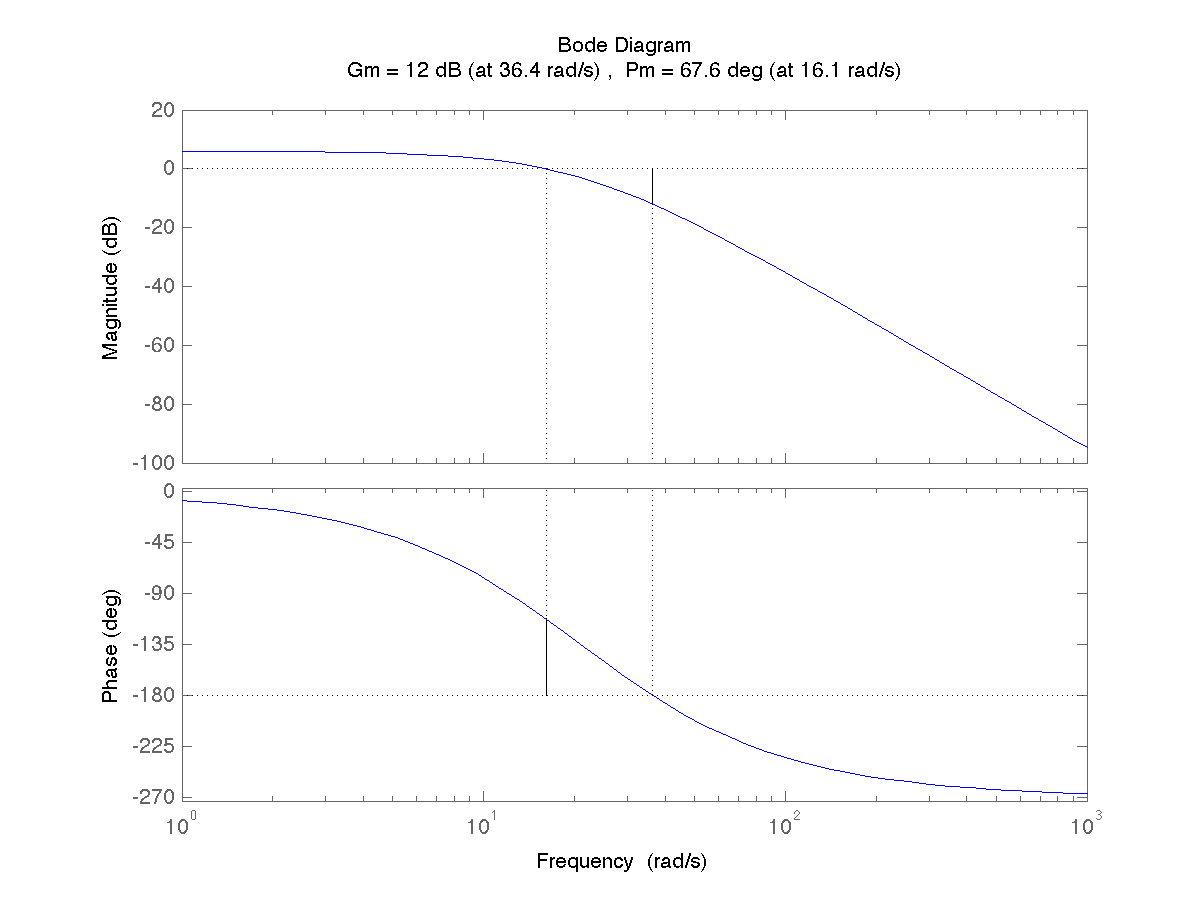
\includegraphics[width = \linewidth]{part4_analog.png}
\label{fig:4_a1}
\end{figure}

\begin{figure}[h!]
\caption{Black Box Digital System $K_u$ = $6.47dB$ =2.1 $T_u$ = .2371s} 
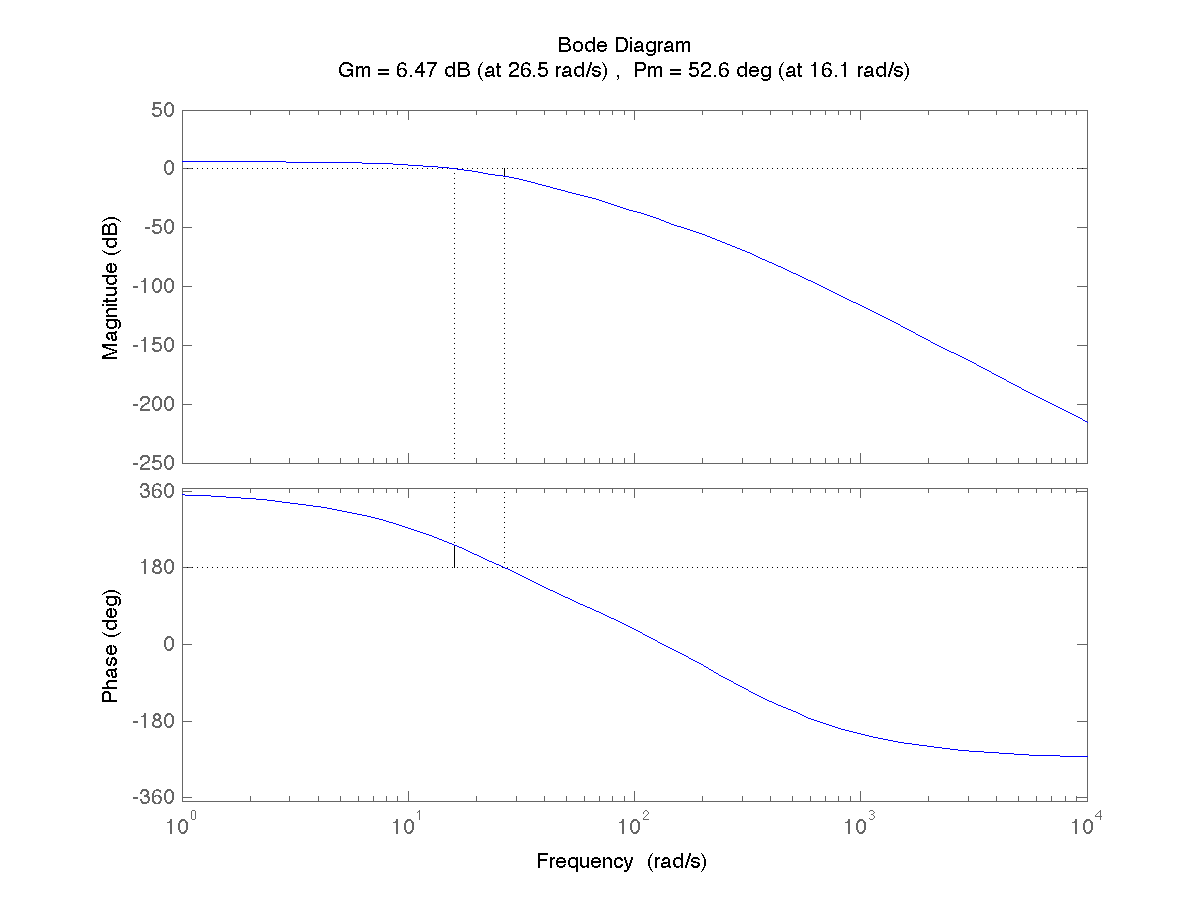
\includegraphics[width = \linewidth]{part4_digital.png}
\label{fig:4_a2}
\end{figure}
\FloatBarrier 

\subsection*{Use Ziegler Nichols}

\begin{figure}[h!]
\caption{Black Box Analog System Cross over Frequency =39.2 rad/s} 
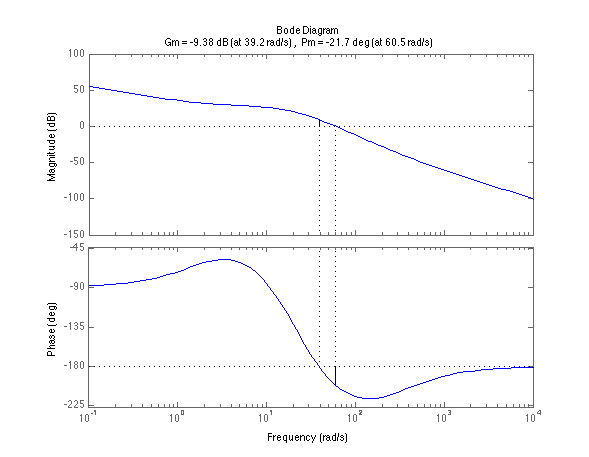
\includegraphics[width = \linewidth]{4b_analog.png}
\label{fig:4_b1}
\end{figure}

\begin{figure}[h!]
\caption{Black Box Digital System Cross over Frequency = 28.4 rad/s} 
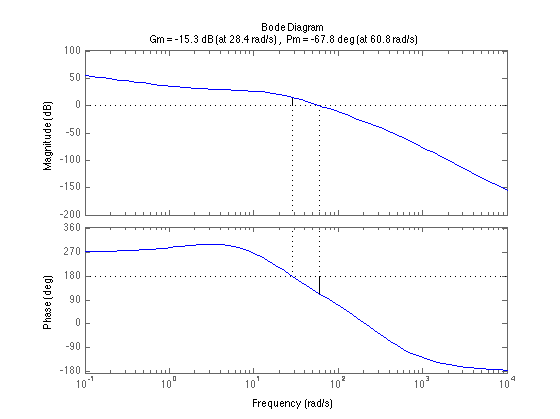
\includegraphics[width = \linewidth]{4b_digital.png}
\label{fig:4_b2}
\end{figure}
\FloatBarrier

\subsection*{Discuss the margins for the nominal design.}
Since 0dB gain is past the 180 phase frequencies for both we should adjust the gains to have the crossover  frequency less than the 180 margin frequency. 
 
 \begin{figure}[h!]
\caption{Black Box Analog System Adjusted Gains} 
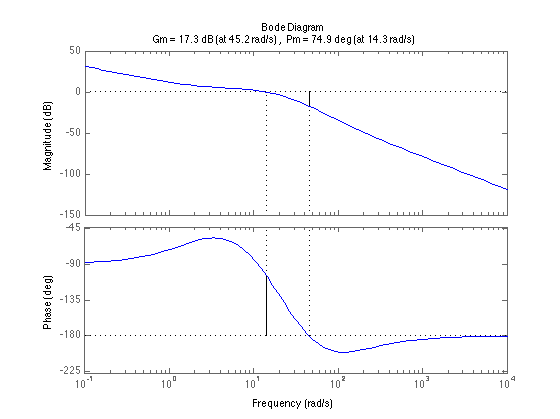
\includegraphics[width = \linewidth]{4c_analog.png}
\label{fig:4_c1}
\end{figure}

\begin{figure}[h!]
\caption{Black Box Digital System } 
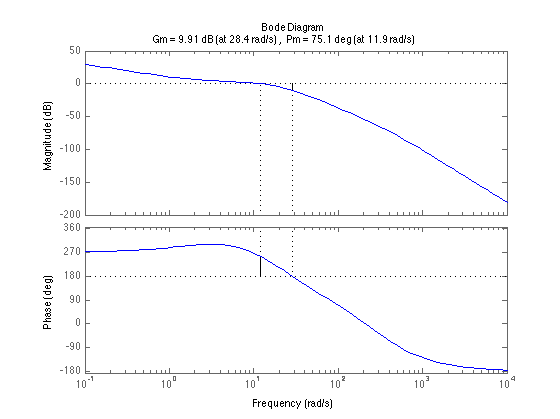
\includegraphics[width = \linewidth]{4c_digital.png}
\label{fig:4_b2}
\end{figure}
\FloatBarrier

\section*{12 Red Blue}

\end{document}
